\documentclass[thesis.tex]{subfiles}

\begin{document}

% ----------------------------------------------------------
\chapter{Methodology} \label{chap:methodology}
% ----------------------------------------------------------
% Present the method and system. Basically write everything you've done.
% ----------------------------------------------------------
In this chapter we will discuss how we created the dataset used in our research, what the dataset contains and the purpose for which we created it. 




% ----------------------------------------------------------
\section{Data collection} \label{sec:data_collection}
% ----------------------------------------------------------
% Present how you gathered the data and labels
% ----------------------------------------------------------
As discussed in Section \ref{sec:available_datasets} there is number of publicly available datasets online, and some which are restricted. Some of these datasets are difficult to access, and there is a need for more publicly available datasets which are collected for the purpose of deep learning. To assist the under-explored field of research within medical computer assisted analysis tools the datasets need to be large and well annotated. Some of the mentioned datasets lack adequately documented, annotated samples from a good source and is not well suited for our research. Thus, as a vital part of our research, we aim to produce a collection of well annotated and adequately big dataset that can be used not only in this study, but also contribute to the research community and have a impact on the research comparability in future. We achieve this by collecting medical data, sorting and annotating it and making the dataset publicly available and free for non-commercial, educational and research purposes.


\subsection{Privacy, Legal and Ethics Issues}
%Source: pogorelov thesis 3.1.1
% ----------------------------------------------------------
To obtain medical videos from a hospital in Norway is very difficult and not straight forward. All medical data is considered personal and is therefore strongly protected from unauthorized use and distribution by the \textbf{Pasientjournalloven??} legislation.
A medical study conducted at 2 academic hospitals from May 2017 to September 2018 found that most patients are willing to share their data and biospecimens for research purposes \cite{PatientPerspectives19}. Regardless of the patient opting in to share their data and biospecimens it is difficult for researchers to get their hands on it. 
%TODO : why is it difficult to access data?
We solved this problem by collaborating with a number of Norwegian hospitals and research teams working there. One of the research teams we collaborated with is Augere Medical (See Section \ref{sec:augere_medical} for more info), and through them we got in contact with Vestre Viken Hospital Trust, allowing our research team to download anonymous data from hospital systems and transfer it using secure media to our facility. Upon downloading the data we further stripped the metadata files for potential information regarding patients like time stamps, dates and camera equipment used.
%TODO : ethics?

% From ds-paper
% The study was approved by the Privacy Data Protection Authority.  It was exempted from approval from the RegionalCommittee for Medical and Health Research Ethics - South East Norway. Since the data is anonymized, the dataset is publiclyshareable based on Norwegian and General Data Protection Regulation (GDPR) laws.



\subsection{Hyper-CasuleCam} \label{sec:hyper-capsulecam}
% Where is the dataset collected from?
% ----------------------------------------------------------
The dataset we used in our experiments consist of endoscopic videos collected from Bærum Hospital, a hospital in Vestre Viken Hospital Trust. Unlike Kvasir V2 and Hyper-Kvasir datasets we have made the Hyper-CasuleCam dataset for the purpose of this thesis. Initially we received 44 VCE videos, which were first reviewed by a clinician, whom selected thumbnails of region of interests of both lesions and normal findings. The videos were then exported from Vestre Viken Hospital Trust and re-encoded to an open source file format (MP4?), from proprietary Sony technology format (whats the name?) %TODO what format?
Prior to being exported the videos were anonymized by removing all metadata and renaming the files with randomly generated file names. A few videos had to be shortened to cut out images taken by the capsule before entering the mouth of the patient. After that the videos are uploaded to Augere Medical AS\footnote{\url{https://augere.md/}} tagging tool. Three MSc students went through all the frames of the videos in collaboration with an expert and labeled and marked findings with bounding boxes. When the student encountered images they were uncertain of the expert reviewed the case.

There are a total of XX different findings in the dataset. The findings are split in two different types; anatomical landmarks and pathological findings. Anatomical landmarks consist of two categories:
\begin{itemize}
\item Pylorus valve; where the capsule enters the small intestine from the stomach.
\item Ileocecal valve; the transition from small intestine to large intestine. 
\end{itemize}

Pathological findings consist of:
\begin{itemize}
\item Protruding lesions; polyps, varices and tumors.
\item Excavated lesions; scars, ulcers, erosions, angiectasia, and dieulafoy lesions.
\item Mocusa; edematous, scalloping, hemorrhagic, erythematous, and ulcerated mucosa.
\item Normal; no pathological finding.
\end{itemize}

We have also included one category for foreign bodies which includes images with things found inside the small intestine which does not fit in any of the previously mentioned categories. This includes thing like other VCE-devices and tables. The images annotated with the \textit{normal} tag is meant to be used for binary classification where all the others classes are combined into a single class for \textit{finding} and one class for no findings. \textit{Normal} images are hand picked from portions of video where there are no findings, and taken from each video to get a diverse category.

When all 44 videos have been precisely labeled the dataset is exported from Augere Medical tagging tool and split into folders for each class. The number of images per class are given in Table \ref{table:kvasir_pillcam_samples} and Figure{fig:hyper-capsulecam-dist} with an algorithmic scale. In total we have 43,905 labeled images in 12 classes. The sample distribution across the classes is skewed depending on how many findings there are in the videos. Some findings occur often and some very rarely. 

\begin{figure} % fig:hyper-capsulecam-dist
  \begin{center}
    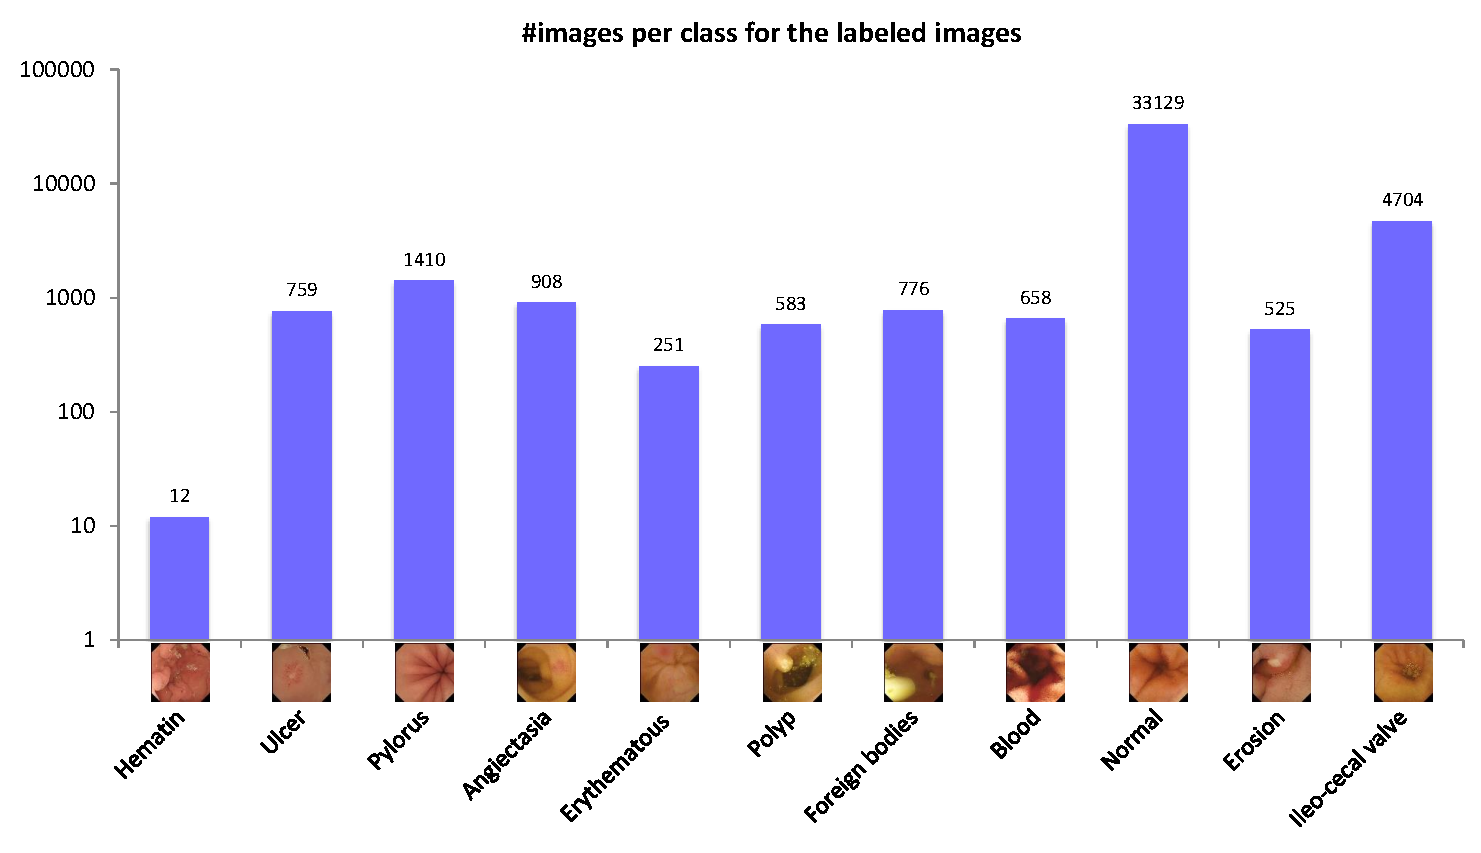
\includegraphics[width=1.0\textwidth]{hyper-capsulecam-dist}
    \caption[Naive pipeline.]{The time spent for reading, opening and training - the naive method.}
    \label{fig:hyper-capsulecam-dist}
  \end{center}
\end{figure}

Imbalanced dataset pose a challenge for predictive algorithms as most learning algorithms are based on the assumption of an equal number of samples for each class. This results in models that have poor predictive performance, especially for minority class or classes. This is a great problem because in many medical datasets the minority class is the most important and therefore more sensitive for classification errors.

In addition to labeling the images the dataset also contain a JSON format file which stores coordinates for where in the frame the finding is located. The Kvasir-PillCam dataset will be an open-source dataset available for others scientists, and will later be grown to include more PillCam videos, both labeled and unlabeled samples.

%TODO : update this table with the final classes and numbers
\begin{table} % table:kvasir_pillcam
  \centering
  \begin{tabular}{|l|r|l|}
  	\hline
  	Class name & \# samples & Percentage \\
    \hline
    Angiectasia		& 908	& xx,x \\ 
    Blood			& 658	& xx,x \\ 
    Erosion			& 525	& xx,x \\ 
    Erythematous	& 251	& xx,x \\
    Foreign Bodies	& 776	& xx,x \\
    Hematin			& 12	& xx,x \\
    Ileo-cecal valve& 4704	& xx,x \\
    Normal			& 33,129& xx,x \\
    Polyp			& 583	& xx,x \\
    Pylorus			& 1410	& xx,x \\
    Ulcer			& 759	& xx,x \\
    Unknown			& 190	& xx,x \\
    \hline
  \end{tabular}
  \caption{Hyper-PillCam class names, corresponding amount of samples and the percentage of samples in each class.}
  \label{table:kvasir_pillcam_samples}
\end{table}

Later, we received an additional XX videos. These videos were not annotated but used for unlabeled data. (and/or sample-videos?)
These videos were processed exactly the same as previous videos, so that it will be compatible (**describe**) with the annotated dataset.


\subsubsection{Labeled images}
\subsubsection{Unlabeled images}
\subsubsection{Videos}

% ----------------------------------------------------------
\section{Data pipeline} \label{sec:data_pipeline}
% ----------------------------------------------------------
% Present everything related to working with data files
% tensorflow.data.Dataset pipeline with prefech, batching, shuffling, caching etc
% ----------------------------------------------------------
The preprocessing pipeline is implemented by using TensorFlows \textit{data.Dataset} library. This was chosen over \textit{datagenerator} due to the easy of use, but later became an issue due to the complexity and some diffuse runtime errors. The main benefits by using data.Dataset is that all data is handled in tensors and computation is automatically distributed to the GPU which enhance the load distribution of processing power. 

The pipeline outline can be seen in Figure XX.
%TODO add figure of data pipeline and describe each step and why its done


All the code for handling the data pipeline is managed in a separate script called pipeline.py. Psuedo code for the script is:
%TODO : add code outline / psuedo code



\subsection{Splitting and resize images}
% could also be called 'image preprocessing'?
% ----------------------------------------------------------
Although not strictly a part of the pipeline itself the preprocessing is a vital step in machine learning as the quality of the data and the useful information that can be derived from it directly affects the ability of our model to learn.

Initially the dataset was split into three; training data, test data, and validation data. This was done by using tf.data.Dataset core operations \textit{take} and \textit{skip}. The take function, when called upon, returns a sub-dataset with the same number of samples as the number it receives as a argument. Skip function returns a sub-dataset where it skips the number of elements as stated in input argument and return the remaining samples.

\begin{lstlisting}[language=Python]
>>> dataset = tf.data.Dataset.range(10)
>>> dataset = dataset.skip(7)
>>> list(dataset.as_numpy_iterator())
[7, 8, 9]
\end{lstlisting}

However, because of the imbalanced dataset we have been working with this turned out to drop minority classes in some runs. This happened because the take and skip methods picks samples from the entire dataset as whole, and not per class. In Hyper-Kvasir the class with smallest number of samples, called a minority class, is hemorrhoids with 6 samples. Depending on the random shuffling for each run these samples would often all end up in one of the dataset splits and not be represented in the other two.
%Discovered non-optimal implementation of dataset splitting, which left some of the most vulnerable minority classes with no samples in the test data. 
To mitigate this issue I created a separate script for pre-splitting dataset into sub folders for each, training, testing and validation dataset. The outline of this script is given below.

\begin{lstlisting}[language=Python]
for every class name in directories:
	sort the images
	shuffle the filenames
	split the class into train, test and val
	for each split_ds in datasets:
		for filename in sub-split:
			resize and save the image
\end{lstlisting}

We split the data into 60\% training data, and leave 15\% for test data and validation data respectively. To make the split reproducible we first sort the data in alphabetically order after file names then use seeded random to shuffle the filenames so the three datasets contains a random assortment of images from the original dataset. 
In this step we also reduce the image dimensions to 256 by 256 pixels to make the data easier to use during the next preprocessing steps. For downscaling the images we use a \textit{resize} function from the highly optimized library openCV's, with a bilinear interpolation. We used openCV because for this particular task it was about 30\% faster than Pillow, another popular Python imaging library. However this downscaling might introduce aliasing and artifacts to the images as the Hyper-Kvasir's median image dimensions are 768 by 576 pixels, which means we are reducing the dimensions with a factor of three. Area based interpolation \cite{AreaBased99} or Gaussian resampling, with a suitable chosen radius, may give better results. This is something I would like to have tested if I had more time.

Another benefit we get from running all images through this processing script is the reduction in dataset file size. In Hyper-Kvasir this size reduction correspond to a magnitude in total file size reduction, from 28 gigabytes to 2.8 gigabytes. This helps to efficiently load the images into the pipeline during training.

At this step it would be natural to also apply normalization to the images, but TensorFlow handles this gracefully while reading the images from disk, so we have opted to leave this out of the script. To normalize an image in the context of machine learning means to squeeze the pixels values into a range from zero to one. This is done because usually when reading an image from disk it is represented with an integer value between 0 and 255. Although this integer value can be directly represented to the neural network models, this can result in challenges during training like slower learning.

Finally the images are saved to a corresponding directory for each train, test and validation data in the given output directory.


\subsection{Loading images into the pipeline}
% write about the first part of create_dataset script
% ----------------------------------------------------------
To efficiently read and process the images in the pipeline we use TensorFlow's function \textit{list\_files} from the tensorflow.data API. This function creates a Python iterable dataset object of all files matching a glob pattern. An example of a glob pattern could be "/source/datasets/*.jpg". In this example the "*.jpg" is a wildcard followed by a image format extension, which means that a dataset will be created out of all jpg images inside the "datasets" directory. This function then returns a dataset of strings corresponding to filenames. Although not strictly necessary because the images were randomly shuffled before being split into train, test and validation datasets, the filenames are shuffled again upon entering the dataset. This is repeated three times for each of the train, test and validation datasets. If we get 5 samples from this dataset of strings this is how they would be represented:

\begin{lstlisting}[language=Python]
>>> for path in dataset.take(5):
>>> 	print (path)
tf.Tensor(b'/data/normal-cecum/cc6ed77fbc04.jpg', shape=(), dtype=string)
tf.Tensor(b'/data/polyps/119100adf1de.jpg', shape=(), dtype=string)
tf.Tensor(b'/data/esophagitis/f3be6279f5f7.jpg', shape=(), dtype=string)
tf.Tensor(b'/data/dyed-lifted-polyps/cbdfb00c142d.jpg', shape=(), dtype=string)
tf.Tensor(b'/data/dyed-lifted-polyps/b1aa0268867b.jpg', shape=(), dtype=string)
\end{lstlisting}

Next we apply a transformation function to each element of the dataset to create (image, label) pairs from the filepaths. This transformation function does three things; one-hot encodes the label based on the parent directory; decodes the image so the image is represented with a tensor with dimensions (image width, image height, color channels); resize the image to the correct dimensions. 

Once we have a dataset object we can transform it into a new dataset by chaining method calls on the dataset object.


\subsection{Optimize performance}
%source1: https://www.tensorflow.org/guide/data_performance#optimize_performance
%source2: https://www.tensorflow.org/api_docs/python/tf/data/Dataset#cache
% ----------------------------------------------------------
To build a efficient pipeline it is required that the Graphical Processor Unit (GPU) is fed data at the right time. If the GPU is waiting to receive data the pipeline is not optimized and training will take longer. Preferably the pipeline delivers data for the next step before the current step has finished. 

The main steps involved in training a model is (1); opening a file, (2); reading the data from that file and (3); using the data for training. If these operations are performed in synchronous and sequential order the model can not train while it is waiting idle for an image to be opened and read. Therefore the training step time is the sum of all three steps, see Figure \ref{fig:pipeline_naive}. 

\begin{figure} % fig:pipeline_naive
  \begin{center}
    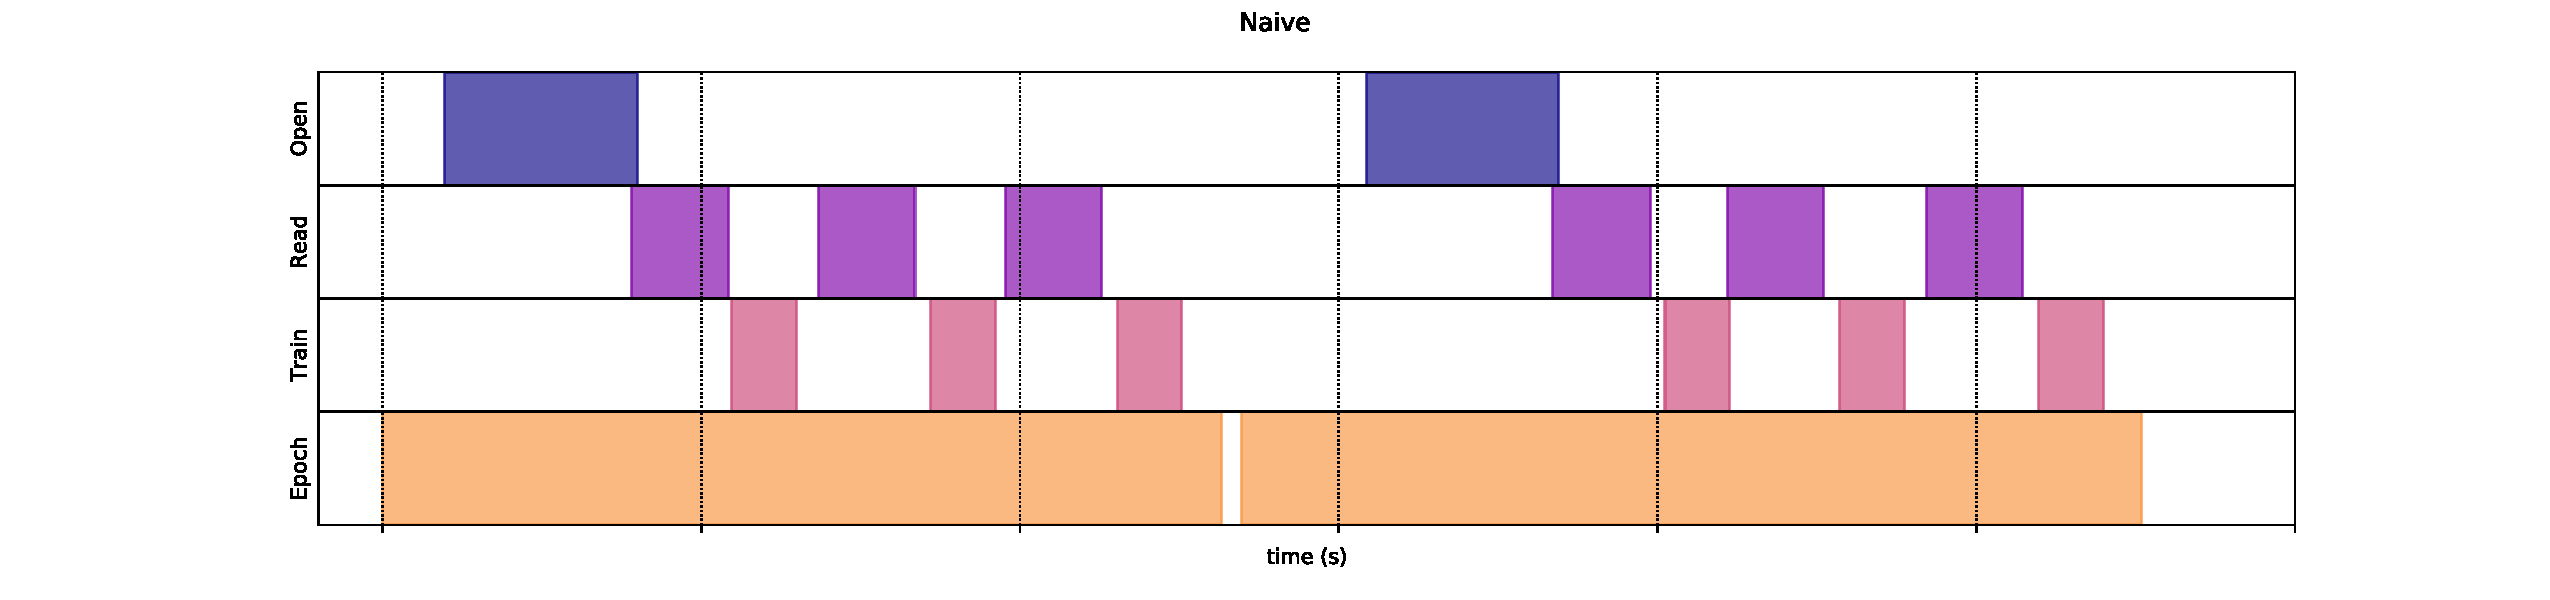
\includegraphics[width=1.0\textwidth]{pipeline_naive}
    \caption[Naive pipeline.]{The time spent for reading, opening and training - the naive method.}
    \label{fig:pipeline_naive}
  \end{center}
\end{figure}

To mitigate this time-consuming issue the tf.data API have a couple of tools at disposal. The first one is prefetching. 
Prefetching overlaps the preprocessing and model execution of a training step. While the model is executing training step $s$, the input pipeline is reading the data for step $s+1$. Doing so reduces the training step time by a significant amount as seen on Figure \ref{fig:pipeline_prefetch}.
Because we are using a tf.data.Dataset object for holding all our images it is very easy to introduce prefetching to the pipeline. The tf.data API provides the tf.data.Dataset.prefetch transformation which decouple the time when data is produced by the CPU from the time when data is consumed by the GPU. 

\begin{figure} % fig:pipeline_prefetch
  \begin{center}
    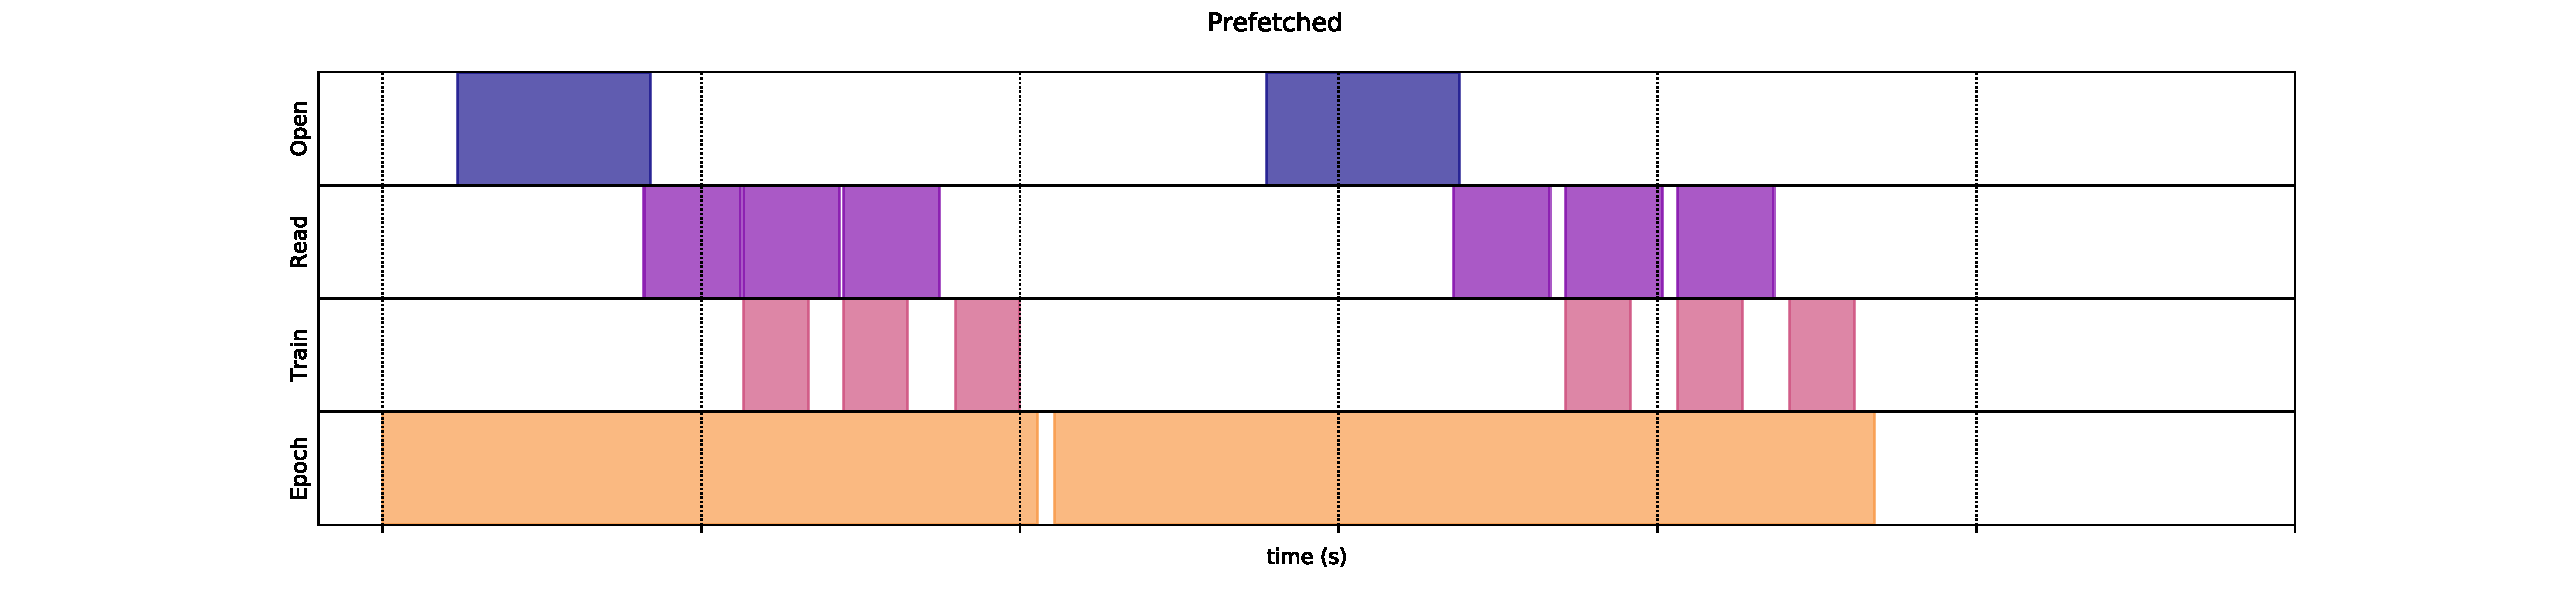
\includegraphics[width=1.0\textwidth]{pipeline_prefetch}
    \caption[Pipeline with prefetching.]{Time spent on reading, opening and training with pipeline prefetching enabled.}
    \label{fig:pipeline_prefetch}
  \end{center}
\end{figure}

We rely heavily on data augmentation to help the model to generalize and not overfit. This is done when preparing the data by using tf.data.Dataset.map transformations, which applies a user-defined function to each element of the input dataset. Because the samples are independent of one another, the process can be parallelized across multiple CPU cores. The tf.data API provides a num\_paralell\_calls argument to specify the level of parallelism, this argument can be set manually or automatically. We have chosen to go with the automatic delegation, which sets the level of parallelism on runtime. See Figure \ref{fig:pipeline_sequential} for the naive approach, and Figure \ref{fig:pipeline_parallel_map} for overhead when using parallel mapping.

\begin{figure} % fig:pipeline_sequential
  \begin{center}
    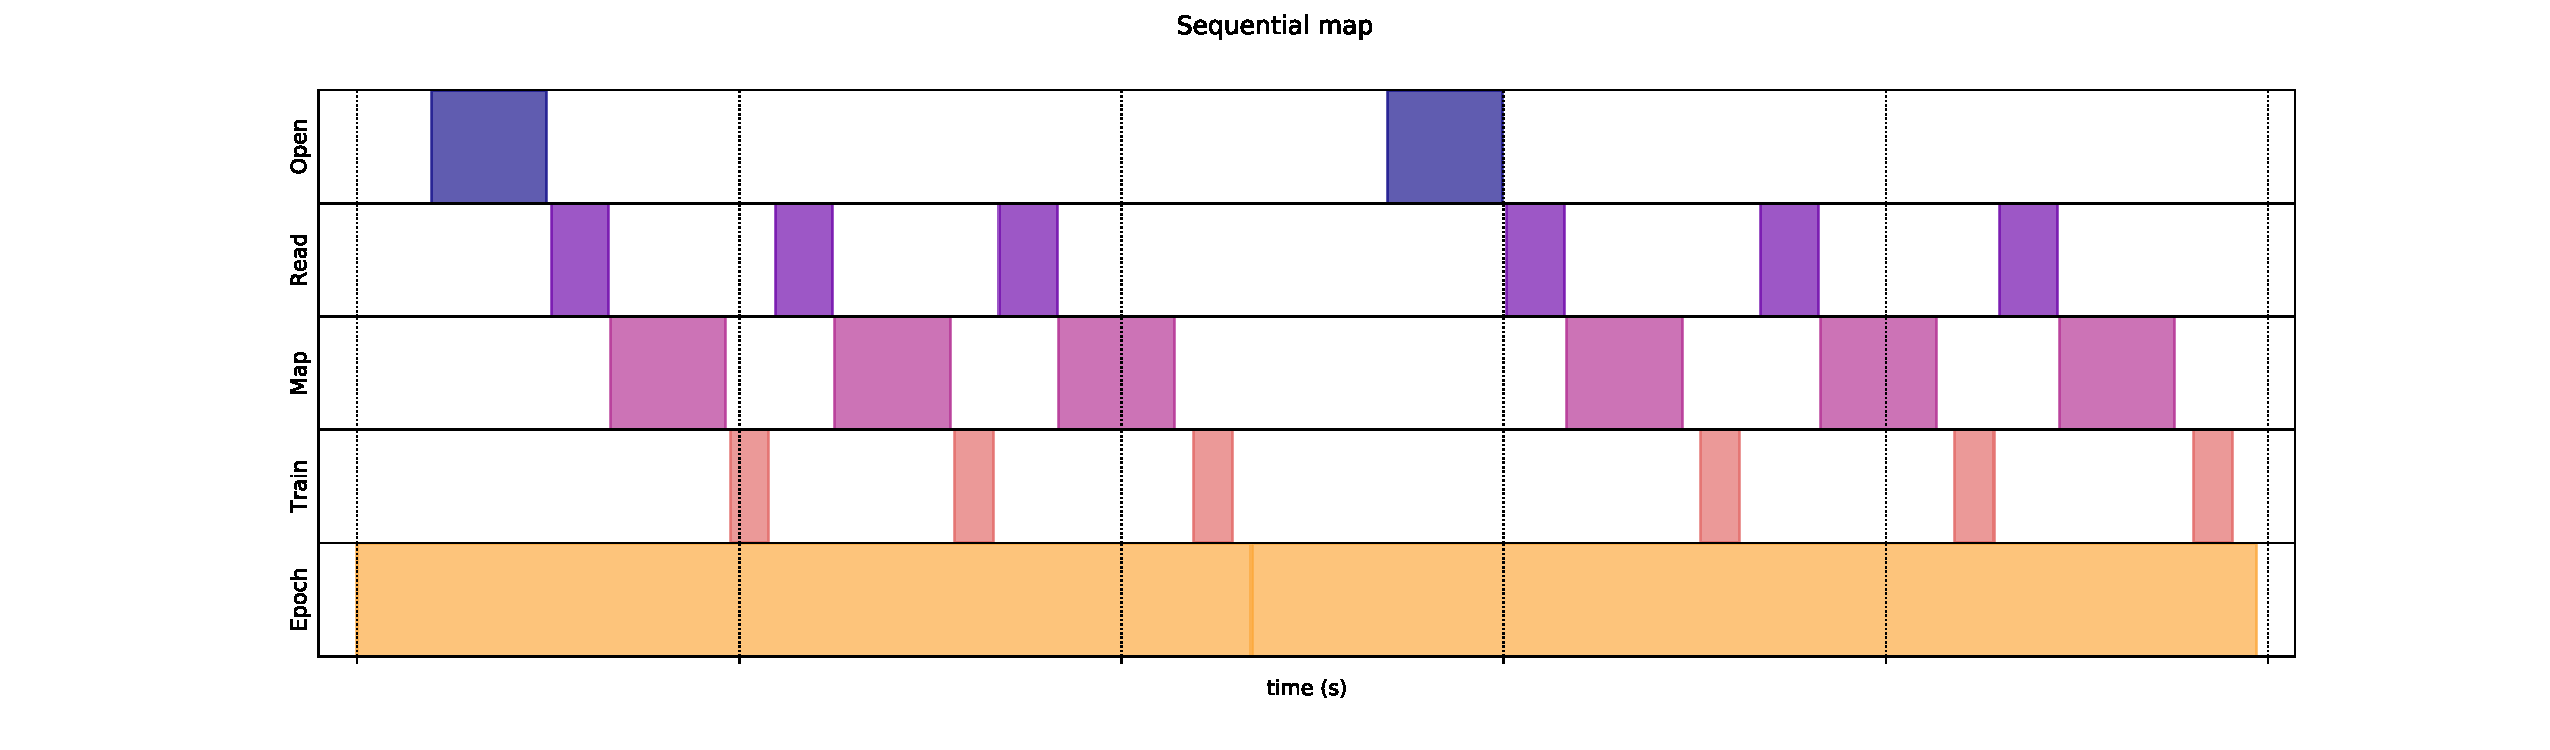
\includegraphics[width=1.0\textwidth]{pipeline_sequential}
    \caption[Naive pipeline with mapping.]{Naive pipeline, here the times spent on opening, reading, pre-processing and training steps sum together for a single iteration.}
    \label{fig:pipeline_sequential}
  \end{center}
\end{figure}

\begin{figure} % fig:pipeline_parallel_map
  \begin{center}
    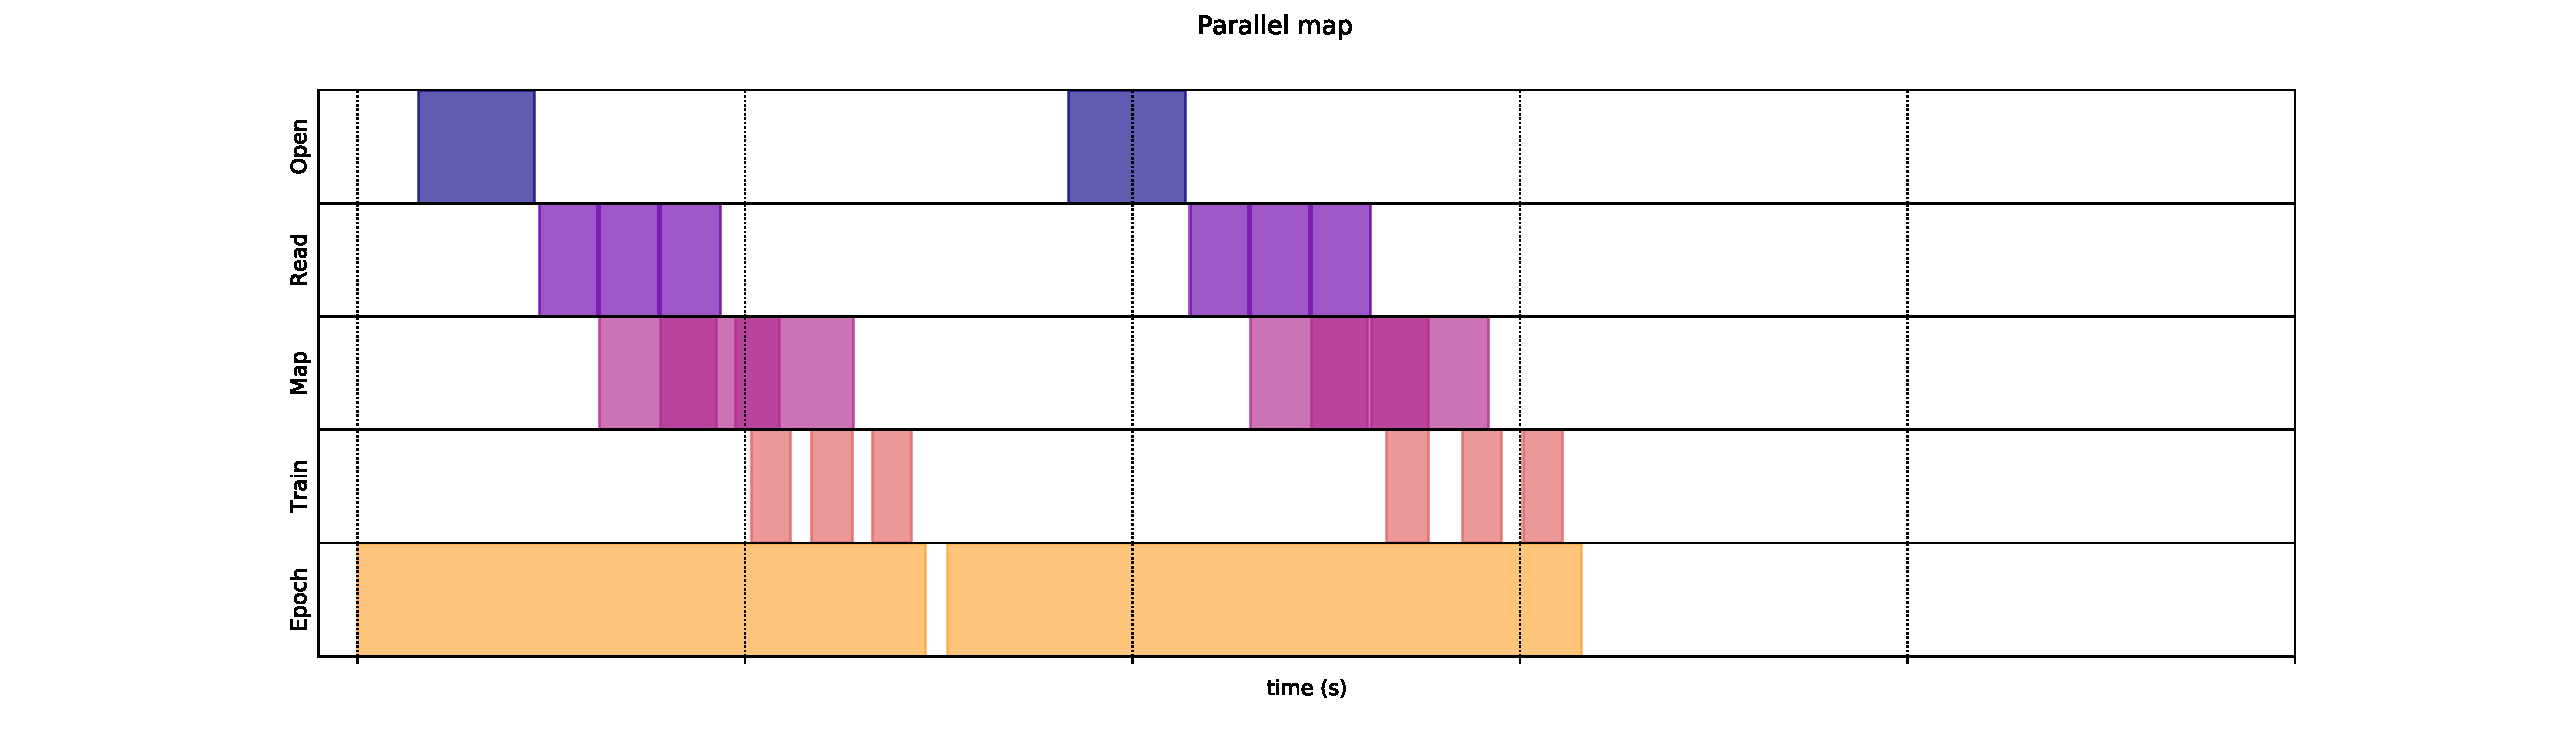
\includegraphics[width=1.0\textwidth]{pipeline_parallel_map}
    \caption[Pipeline with parallel mapping.]{Here you can see pre-processing steps overlap, and the overal time for each iteration is reduced.}
    \label{fig:pipeline_parallel_map}
  \end{center}
\end{figure}

The last step we take to optimize the training efficiency is to cache the dataset to local storage (an NVMe SSD in our case). 



\subsection{Shuffle the dataset}



\subsection{Repeat}



\subsection{Data augmentation}
What is the necessity of rotating the samples. Will they not always be 'square'?



\subsection{Batching}



\subsection{Sample the dataset or class weight}
Found that when weighting the classes the model learns slower. Which means decay rate of learning rate must be lowered for it not to drop too soon. Also increase the buffer for early stopping of training.

%TODO add formula for calculating class weights



\subsection{Training}
%TODO Include a table of computer hardware used for training, and versions of all libraries used (like hicks p.73

Normalization; any benefit of using L2 normalization in last dense layer when using a pre-defined model?

% ----------------------------------------------------------
\section{System implementation} \label{sec:system_implementation}
% ----------------------------------------------------------
% Present the system architecture, some results perhaps
% ----------------------------------------------------------


\subsection{Generating new pseudo labels}
When we use the trained teacher model to generate new pseudo labels from the dataset we set a threshold for which the predicted image is saved if it is above the set value. Here we have two options, either to set the threshold low and extract a large dataset with high uncertainty, but get the most of our minority classes. Or we can set the threshold high, and gather a dataset with lower uncertainty, but might miss more samples for the minority classes.

After subtracting samples from the unlabeled dataset through predicting and saving images with a probability score higher than the threshold, we sort the images based on the probability scores. This is done so for majority classes with a large amount of samples can be squeezed to fit the minority classes and we can select the samples with the highest probability scores.

The sorted samples from the unlabeled dataset is then resampled based on the original distribution of samples in the training data. Since the original dataset is resampled that means we will pick out X samples for each class to keep the distribution even between classes during training.

\subsubsection{Inspecting the pseudo labels}
Since the unlabeled dataset don't contain labels, it is difficult to fully comprehend the results of the extracted data.
%TODO mention that the result are checked with a specialist
%TODO add figure of unlab_ds_checkout-all.pdf



\subsection{Learning rate}
% see https://www.tensorflow.org/tutorials/keras/overfit_and_underfit
Many models train better if you gradually reduce the learning rate during training. We are using learning rate which follows a inverse time decay which means that the learning rate is decreased to 1/2 of the base rate at 10 epochs, 1/3 at 20 epochs and so on.

%TODO add plot of impact of decay rate and explain


\subsection{Hyper-parameter tuning}





% ----------------------------------------------------------
\section{Summary} \label{sec:C3-summary}
% ----------------------------------------------------------
% Present a summary of the chapter
% ----------------------------------------------------------


\end{document}